\documentclass[presentation]{beamer}
\usepackage{isac-slides}
\usepackage{minted}

\title[Simulation]{Stochastic Simulation in Alchemist}

\begin{document}

\frame[label=coverpage]{\titlepage}

\newcommand{\ov}[1]{\(\overline{\texttt{#1}}\)}
\newcommand{\pedix}[1]{\({}_{\texttt{#1}}\)}
\newcommand{\apedix}[1]{\({}^{\texttt{#1}}\)}
\newcommand{\p}[0]{\('\)}
\newcommand{\xt}[1]{\texttt{#1}}
\newcommand{\bnfs}[0] {\;|\;}
\newcommand{\opar}[0] {\,||\,}
\newcommand{\temp}[1] {#1}

\begin{frame}{Introduction}
 \begin{block}{Goals}
  \begin{itemize}
        \item Understand the need for fast simulators for complex systems
        \item Understand the limitations of classic approaches
        \item Learn a bit of Alchemist
  \end{itemize}
 \end{block} 
 \begin{block}{Methodology}
  \begin{itemize}
        \item From model checking to Monte Carlo
        \item Kinetic Monte Carlo (exemplified with chemistry)
        \item Speed up the Kinetic Monte Carlo
        \item Alchemist: Kinetic Monte Carlo for Pervasive computing
        \item Alchemist's engine
        \item Alchemist's model
        \item Quick tutorial on simulating collective behaviour
  \end{itemize}
 \end{block}
\end{frame}

\section{Simulation and Montecarlo}
\begin{frame}{Model checking: a recap}
 \begin{block}{Pros}
  \begin{itemize}
        \item Complete exploration of the system
        \item Exact verification of property values
  \end{itemize}
 \end{block}
 \begin{block}{Cons}
  \begin{itemize}
        \item In general extremely costly in terms of memory and time
        \item Complexity quickly grows with states
        \item normally only feasible with simple, small systems
  \end{itemize}
 \end{block}
\end{frame}

\begin{frame}{Monte Carlo}
 \begin{block}{Monte Carlo method}
  \begin{itemize}
        \item When it's impossible to explore the whole system
        \item Find a procedure that randomly explores a part of it
        \item Apply it repeatedly
        \item Aggregate the result
  \end{itemize}
 \end{block}
 Trivia: the name is after the famous Casino of Monte Carlo, and refers to the exploration of the probabilities that gamblers can perform by repeatedly play and recording results.
\end{frame}

\begin{frame}{Monte Carlo method and simulation}
	The procedure can POSSIBLY (not compulsorily) be a simulation
	\begin{block}{Example}
		Which is the combined area $A_F$ of these figures?
		\centering
		
\includegraphics[width=0.5\textwidth]{img/mcmethod}
		\pause{}
		\begin{itemize}
			\item Inscribe them within a rectangle of area $A_R$
			\item With a uniform distribution sample $N$ points within that rectangle
			\item Count how many of them are also inside the figures, let this number be $n$
			\item The area of the figures is (approximately) $A_F = \frac{n}{N} A_R$
			\pause{}
			\item This is \emph{not} a simulation
		\end{itemize}
	\end{block}
\end{frame}

\begin{frame}{Simulation}
	\begin{block}{General definition}
		Imitation of the operation of a real-world process or system over time \cite{des-book}.
		\begin{itemize}
			\item Not necessarily run on computers
			\begin{itemize}
				\item e.g. putting a Formula 1 model into a wind tunnel is a sort of simulation
			\end{itemize}
		\end{itemize}
	\end{block}
	\begin{block}{Model}
		The imitation of the real-world process is called \textbf{model}.
		\begin{itemize}
			\item A model is a simplified version of the reality
			\item Simplification is often a requirement, because the original process:
			\begin{itemize}
				\item requires too much time
				\item is not replicable in controlled environments
				\item is too dangerous to replicate
				\item is beyond our technical capacity
			\end{itemize}
			\item Elements relevant to the experiment must be retained in the model
		\end{itemize}
	\end{block}
\end{frame}

\begin{frame}{Types of computer simulation}
	\begin{block}{Time-driven}
		\begin{itemize}
			\item Time is simulated through discrete time slots (ticks)
			\item At every tick, the model is updated to reflect the new state
			\item All the changes occurring during the same tick are considered to be simultaneous
		\end{itemize}
	\end{block}
	\begin{block}{Discrete events (DES)}
		\begin{itemize}
			\item Events are simulated one by one
			\item For every simulated event, the time is shifted forward
			\item Events are strictly ordered: in case two events are scheduled for the same time, one of the two is executed first (and its outcome may influence the remainder of the simulation)
		\end{itemize}
	\end{block}
\end{frame}

\begin{frame}{Kinetic Monte Carlo and chemistry}
Problem: we have a container with a precise number of molecules that may react with each other. We want to forecast the evolution of the system in future.
 \begin{block}{Relax to Continuous}
  \begin{itemize}
        \item In classic chemistry, there are methods based on differential equations to understand the behaviour of such systems
        \item They suppose the concentration of each reactant to be $\in \Re$
        \item It is an approximation: you cannot have a quarter of a molecule!
        \item These methods are accurate only for a high number of molecules
  \end{itemize}
 \end{block}
 \begin{block}{Stochastic simulation}
  \begin{itemize}
        \item What if our system counts few thousands molecules?
        \item Monte Carlo way: let's start with the system in initial state, let it run and see how it behaves. Repeat.
        \item Very hard to do in a real setup: here it comes the simulation
  \end{itemize}
 \end{block}
\end{frame}

\section{Exact stochastic simulation of chemical systems}
\subsection{The problem and a bit of the math behind}
\begin{frame}{Approach the problem}
We need to find a procedure for simulating a chemical system. The system is composed of molecules and reactions. Reactions assume the form:
$$A + B\xrightarrow{\mu} C$$
where $A$ and $B$ are reactants, $\mu$ is an indication of the reaction speed and $C$ is the product.

A solution has been first proposed in \cite{GillespieJPC1977} (Gillespie algorithm or Kinetic Monte Carlo):
 \begin{enumerate}
   \item Select next reaction using markovian rates: it supposes that a chemical system has no memory, and computes the speed of a reaction $r$ as: $a_r = [A][B]\mu$
   \item Execute it, changing the concentrations
   \item Update the markovian rates which may have changed
  \end{enumerate}
\end{frame}

\begin{frame}{Do the math: next reaction choice}
If we assume every reaction is a Poisson process, the probability for it to be the next one is: \\
$$
P(next = \mu)
= \int_0^\infty P(\mu,\tau)d\tau
= \int_0^\infty a_\mu e^{-\tau\sum_j{a_j}}d\tau
= a_\mu \int_0^\infty  e^{-\tau\sum_j{a_j}}d\tau
$$ \\
$$
= -\frac{a_\mu}{\sum_j{a_j}} [e^{-\tau\sum_j{a_j}}]_0^\infty
= -\frac{a_\mu}{\sum_j{a_j}} (e^{-\infty} - e^{0})
= -\frac{a_\mu}{\sum_j{a_j}} (-1)
= \frac{a_\mu}{\sum_j{a_j}}$$
\begin{block}{Details}
 \begin{itemize}
  \item $P(\mu,\tau) = a_\mu e^{-\tau\sum_j{a_j}}$: the probability that the reaction $P$ occurs at time $\tau$ is its speed times the probability distribution. Being this a Poisson process, the probability distribution is a negative exponential function, whose exponent is the sum of the speeds of all the reactions in the system.
 \end{itemize}
\end{block}
\end{frame}

\begin{frame}{Do the math: next reaction time}
We can also compute the next time of occurrence:
$$P(\tau)d\tau = \sum_j P(\mu = j,\tau)d\tau = \left(\sum_j{a_j}\right) e^{-\tau\sum_j{a_j}}d\tau $$
$$ \sum_j{a_j} = \lambda \longrightarrow \lambda e^{-\lambda x}$$
$$F(x\leq t) = \int_{-\infty}^t \lambda e^{-\lambda x} dx = \int_{0}^t \lambda e^{-\lambda x} dx = \left[-e^{-\lambda t}\right]_{0}^t = 1 - e^{-\lambda t}$$
Now, given a uniformly distributed random $\rho$ in $\left[0,1 \right]$, it's possible to compute it's equivalent for the desired distribution:
$$ 1 - e^{-\lambda t} = \rho \Rightarrow t = \frac{-\ln \left( 1 - \rho \right)}{\lambda} \equiv \frac{-\ln \left(\rho \right)}{\lambda}$$
\end{frame}

\begin{frame}{Solve the problem: base algorithm}
 \begin{block}{Algorithm}
  \begin{enumerate}
   \item Set the simulation time $T = 0$
   \item For each reaction $r$ in the whole set of reactions $R$, compute $a_r$.
   \item Select the next reaction $\mu$ to execute. The probability for $r$ to be executed will be $P(r = \mu) = \frac{a_r}{\sum_{(j\in R)} a_j} $
   \item Execute the reaction, changing the concentrations.
   \item Set the simulation time to $T = T_{prev} - \frac{\ln \left( 1 - r \right)}{\lambda}$
   \item GOTO 2
  \end{enumerate}
 \end{block}
 \begin{block}{Data structures}
  \begin{itemize}
   \item Choosing the next reaction to execute can be done by storing in a list like structure reactions and propensities, throwing a random number in $\left[0: \sum_{(j\in R)} a_j\right]$, and selecting the first reaction whose propensity summed to all the previous is equal or higher than the random (linear complexity in time)
  \end{itemize}
 \end{block}
\end{frame}

\subsection{Speed up Gillespie}
\begin{frame}{Speed it up: dependency graph}
 \begin{block}{Algorithm}
  \begin{enumerate}
   \item The propensities must be recomputed at each step, because they depend on concentration of reactants, which may have changed.
   \item However, not every reaction affects the speed of every other: for instance, if $A + B\xrightarrow{\mu_1} C$ executes, the propensity of $D + E\xrightarrow{\mu_2} A$ will not be affected.
   \item We can improve consistently the performance of the algorithm by keeping in memory which reactions influence which other, and updating only those required.
  \end{enumerate}
 \end{block}
 \begin{block}{Data structures}
  \begin{itemize}
   \item A map that connects each reaction to a set of reactions that must be upgraded represents a good dependency graph
  \end{itemize}
 \end{block}
\end{frame}

\begin{frame}{Speed it up: dependency graph}
  \centering
  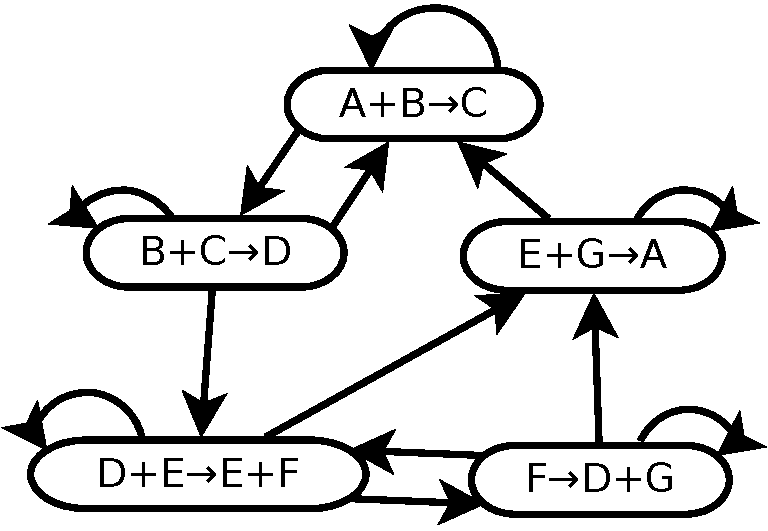
\includegraphics[width=0.89\textwidth]{img/dependencygraph}
\end{frame}

\begin{frame}{Next reaction}
 \begin{block}{Algorithm}
  \begin{enumerate}
   \item Instead of choosing the next reaction probabilistically by propensity, generate a putative time for each reaction.
   \item Sort the reactions by putative time, and take the first.
   \item At each step, for each reaction whose putative time has changed, re-sort the element.
   \item The previous optimization (dependency graph) can be reused.
  \end{enumerate}
 \end{block}
 \begin{block}{Data structures}
  \begin{itemize}
   \item We only need that the first element is the next to be executed.
   \item The best solution is a binary heap*, which can be accessed in O(1) and sorted in log(n), but with a much smaller average complexity.
  \end{itemize}
 \end{block}
 * In the original work \cite{GibsonJPC1999}, the data structure is called ``Indexed priority queue''.
\end{frame}

\begin{frame}{Next reaction: random reuse}
 \begin{block}{Random generation}
  \begin{enumerate}
   \item Generating random number is costly
   \item In a purely chemical simulator, is the most heavy task \cite{GibsonJPC1999}
   \item Reducing the number of generated random numbers is key
  \end{enumerate}
 \end{block}
 \begin{block}{Random reuse}
  \begin{itemize}
   \item Next reaction allows for random reuse
   \item In case the reaction which is being updated is not the one executed but one of its dependencies, then:
   \begin{itemize}
    \item let $T$ be the current simulation time, $\tau_c$ be the new putative time, $a_c$ the new propensity, $\tau_p$ the previous putative time, $a_p$ the previous propensity.
    \item $\tau_c = \frac{a_c \left( \tau_p-T \right)}{a_p}+T$ 
    \item This is possible due to the exponential distribution being \emph{memory less}
    \item Note: $\forall \tau_p, T: \tau_p \geq T $
   \end{itemize}
  \end{itemize}
 \end{block}
\end{frame}

\begin{frame}{Binary heap}
  \centering
  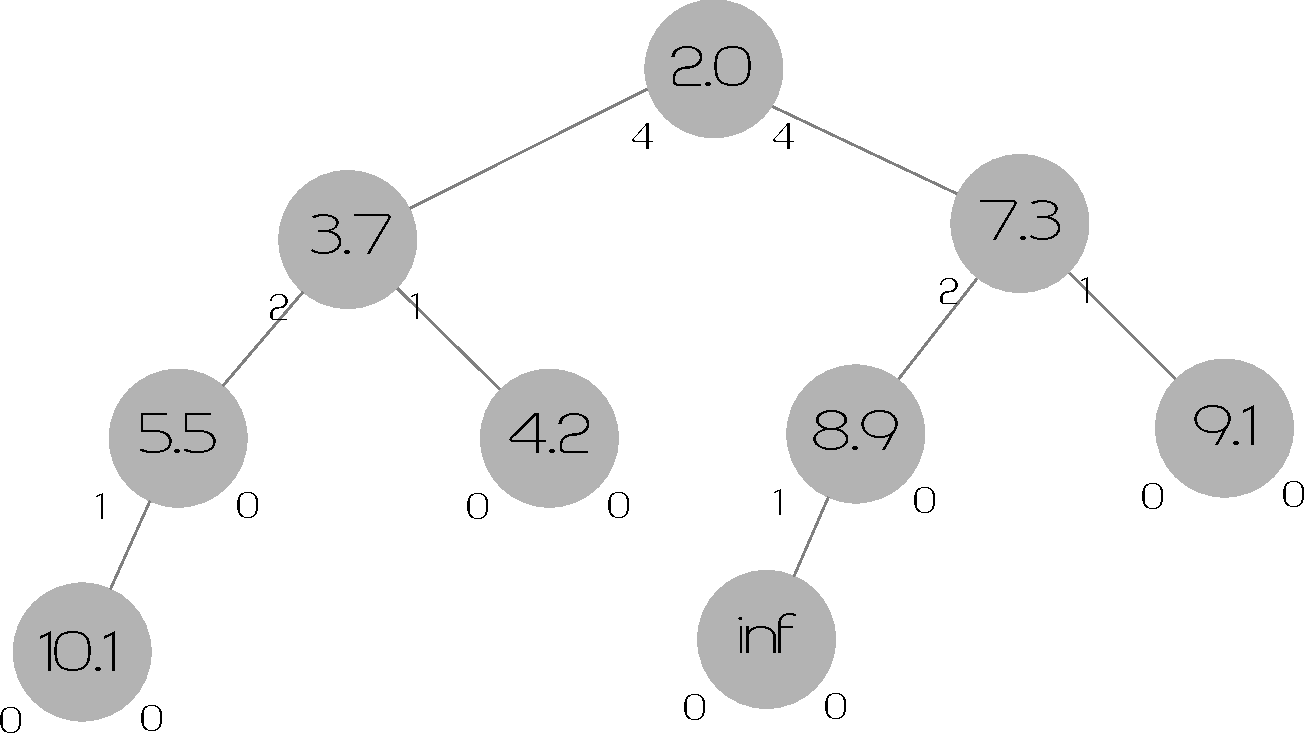
\includegraphics[width=0.99\textwidth]{img/extipq}
\end{frame}

\begin{frame}{Slepoy's Algorithm}
 \begin{block}{Idea}
  \begin{itemize}
   \item Divide the reactions in groups depending on their propensity
   \item Define the groups in such a way that throwing a limited number of randoms the engine can select the next to execute in constant time
   \item Updating the reactions can be done in constant time since the groups have a well defined propensity interval
   \item If the number of groups does not depend on the number of reactions, then the algorithm is O(1).
  \end{itemize}
 \end{block}
 \begin{block}{Drawbacks}
  \begin{itemize}
   \item The algorithm assumes that the number of groups does not depend on the number of reactions, namely, it supposes the propensities to change only a little during the simulation
   \item This assumption is mostly true in real purely chemical systems, but does not hold in general
  \end{itemize}
 \end{block}
\end{frame}

\begin{frame}{Slepoy's Algorithm}
  \centering
  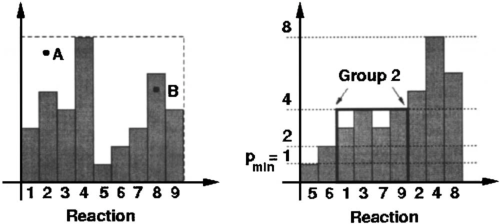
\includegraphics[width=0.99\textwidth]{img/slepoy}

From \cite{SlepoyJPC2008}
\end{frame}


\section{Alchemist}
\subsection{Motivation}
\begin{frame}{From chemistry to pervasive computing}
 \begin{block}{Background considerations}
  \begin{itemize}
   \item Pervasive computing scenarios are normally simulated by means of ``agent based simulators'' (ABS) \cite{wooldridge-intelligentagents}
   \item ABS are extremely flexible, but they lack performance: it's the price to pay for being able to simulate a very wide spectrum of situations
   \item Many pervasive computing scenarios can be modelled as mobile multi-compartmented chemical systems, where molecules are pieces of data (equivalent to a network of Petri Nets)
   \item A whole literature exists on how to make very fast kinetic Monte Carlo algorithms
  \end{itemize}
 \end{block}
 \begin{block}{Idea}
  Instead of use classic ABSs and optimize at the simulation level, can we take a kinetic Monte Carlo and extend it until it supports all the abstractions we need?
 \end{block}
\end{frame}

\begin{frame}{Which scenarios}
 \begin{block}{We want a tool that supports:}
  \begin{itemize}
   \item Self-organising systems
   \item Pervasive computing systems
   \item Crowds of people
   \item Large scale situated systems
   \item Smart Mobility
   \item Crowd detection and steering
   \item Sensor networks
   \item Computational biology
   \item Aggregate programming
  \end{itemize}
 \end{block}
\end{frame}

\begin{frame}{From chemistry to pervasive computing}
 \begin{block}{Requirements}
  \begin{itemize}
   \item Multiple compartments (from now on: nodes)
   \item Molecules can be different data types
   \item Nodes mobility
   \item Non markovian events
   \item More flexible concept of reaction
   \item High performance
  \end{itemize}
 \end{block}
 \begin{block}{Idea}
  Instead of using a classic ABS and optimize at the simulation level, can we take a kinetic Monte Carlo and extend it until it supports all the abstractions we need?
 \end{block}
\end{frame}

\subsection{Engine}

\begin{frame}{Multiple compartments}
 \begin{block}{Extension}
  \begin{itemize}
   \item Up to now we just used a single container with molecules
   \item What if we had multiple intercommunicating containers?
  \end{itemize}
 \end{block}
 \begin{block}{Changes}
  \begin{itemize}
   \item Concept of ``neighborhood'', namely the compartments that can communicate with each compartment
   \item Concept of moving molecules from a compartment to another
   \item Possibly different set of reactions for each compartment
  \end{itemize}
 \end{block}
 \begin{block}{Challenges}
  \begin{itemize}
   \item Who does decide if two compartments are communicating?
   \item How to model a molecule moving towards a new node?
   \item How does the dependency graph change?
  \end{itemize}
 \end{block}
\end{frame}

\begin{frame}{Spatial dependency graph}
 \begin{block}{Challenge}
  \begin{itemize}
   \item There are more reactions: each node has its ``copy''
   \item A reaction may affect the propensities locally, in the neighborhood, or globally 
   \item The fewer are the bindings between reactions, the higher is efficiency of a dependency graph
   \item We want to detect the \emph{context} of the reactions and filter the dependencies accordingly
  \end{itemize}
 \end{block}
\end{frame}

\begin{frame}{Spatial dependency graph}
 \begin{block}{Possible solution}
  \begin{itemize}
   \item Define three contextual levels: \emph{local}, \emph{neighborhood}, \emph{global}
   \item Assign to each reaction an ``input context'', namely which parts of the environment a reaction should read to compute is propensity
   \item Assign to each reaction an ``output context'', namely which part of the environment will be modified by this reaction
   \item A reaction \texttt{r1} may influence a reaction \texttt{r2} if one of the following is true:
   \begin{itemize}
    \item \texttt{r1} and \texttt{r2} belong to the same compartment
    \item \texttt{r1}'s output context is \emph{global}
    \item \texttt{r2}'s input context is \emph{global}
    \item \texttt{r1}'s output context is \emph{neighborhood} and \texttt{r2} belongs to the neighborhood
    \item \texttt{r2}'s input context is \emph{neighborhood} and \texttt{r1} belongs the neighborhood
    \item both \texttt{r1}'s output context and \texttt{r2}'s input context are \emph{neighborhood}, and there is a compartment shared by the two neighborhoods
   \end{itemize}
  \end{itemize}
 \end{block}
\end{frame}

\begin{frame}{Non-markovian events}
 \begin{block}{Example}
   Every second, an external device injects some quantity of molecules within a compartment.
  \begin{itemize}
   \item this event happens precisely every second: it is not a Poisson process!
   \item Its probability distribution id a $\delta$-Dirac Comb
  \end{itemize}
 \end{block}
 \begin{block}{Algorithms}
  \begin{itemize}
   \item The basic Gillespie algorithm is hard to modify to support such events. The main reason is that the choice is not made depending on time, but on propensity, which is an entity strictly bound to the markovian model
   \item The next reaction algorithm, instead, uses putative times: this makes it able to simulate events independently from their distribution, since we just need to correctly estimate the next time of occurrence.
   \begin{itemize}
    \item NOTE: the random reuse is NOT allowed for non-exponential events
   \end{itemize}
  \end{itemize}
 \end{block}
\end{frame}

\subsection{Model}
\begin{frame}{Abstract model}
  \centering
  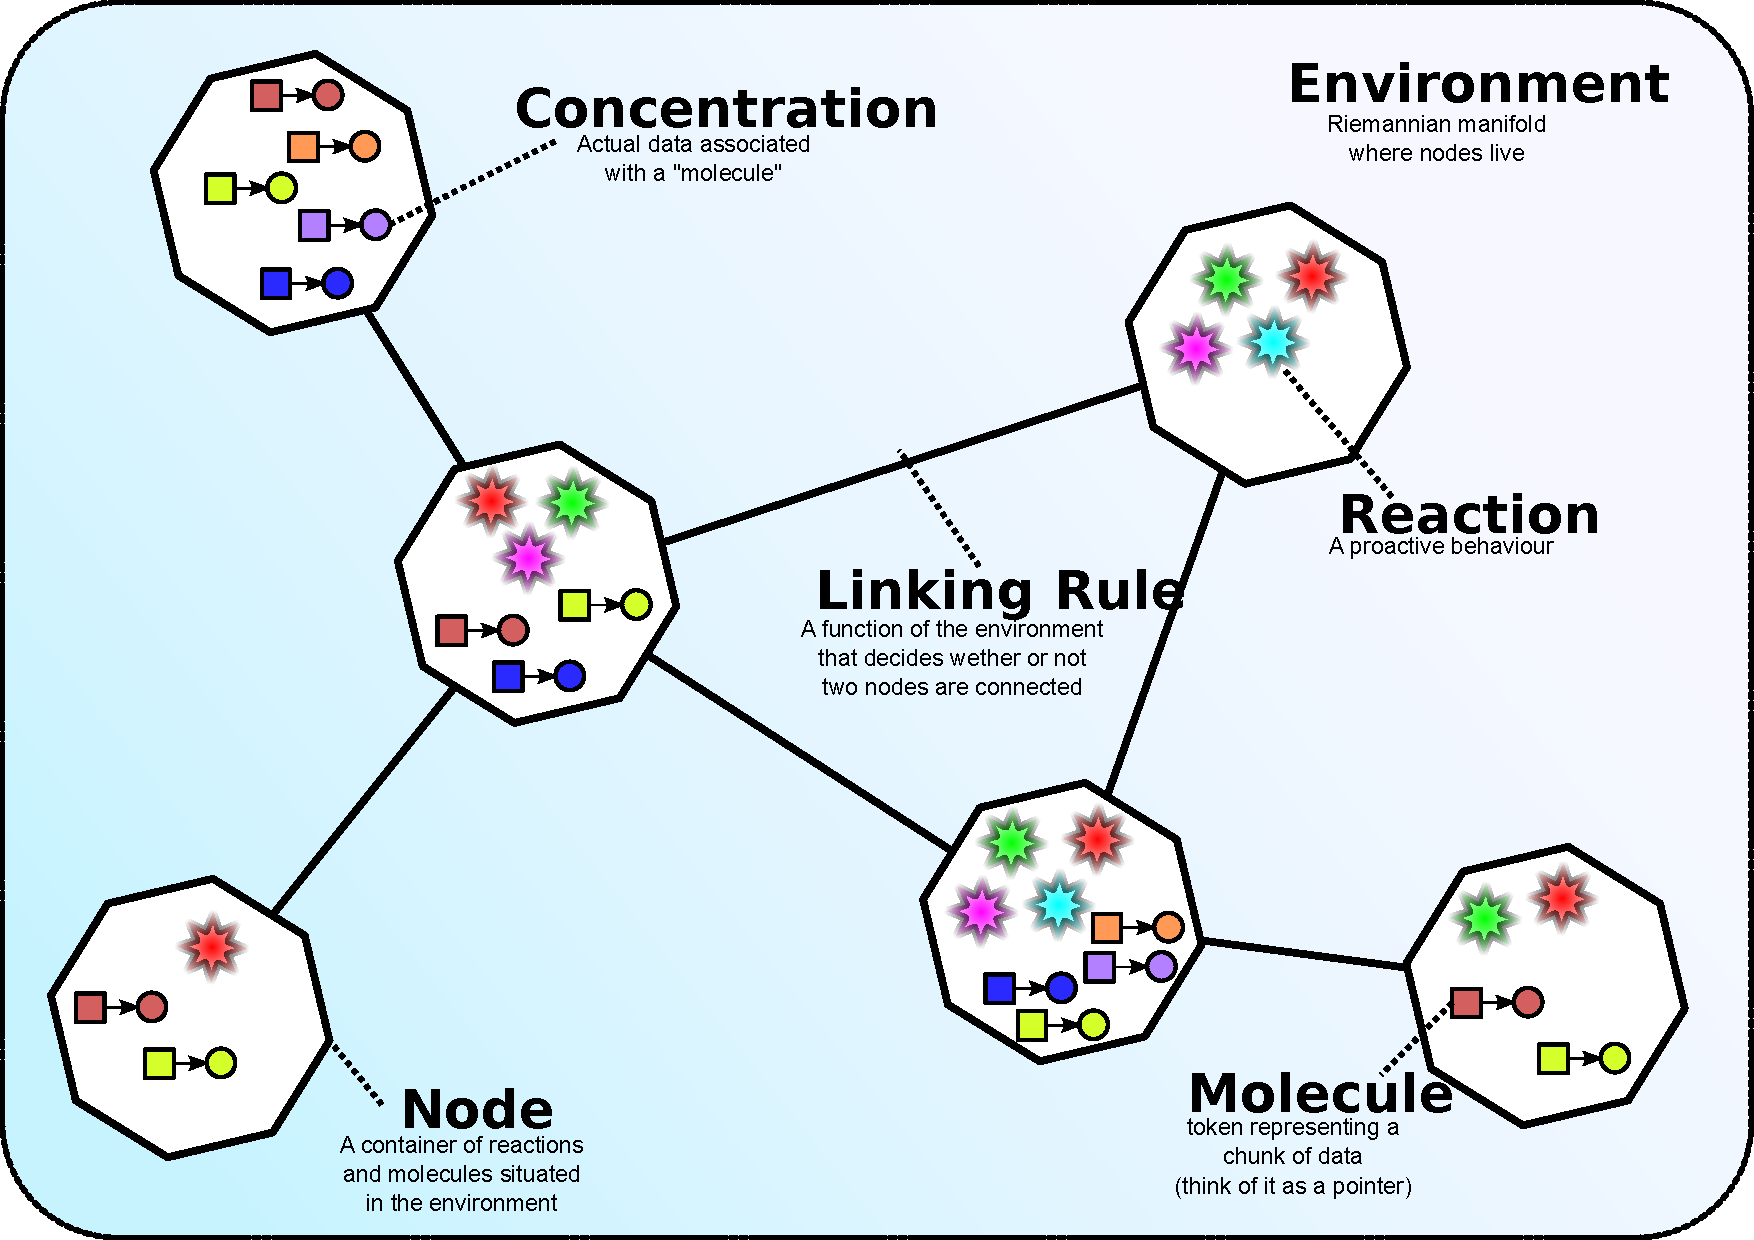
\includegraphics[height=0.85\textheight]{img/model}
\end{frame}

\begin{frame}{Reactions}
  \centering
  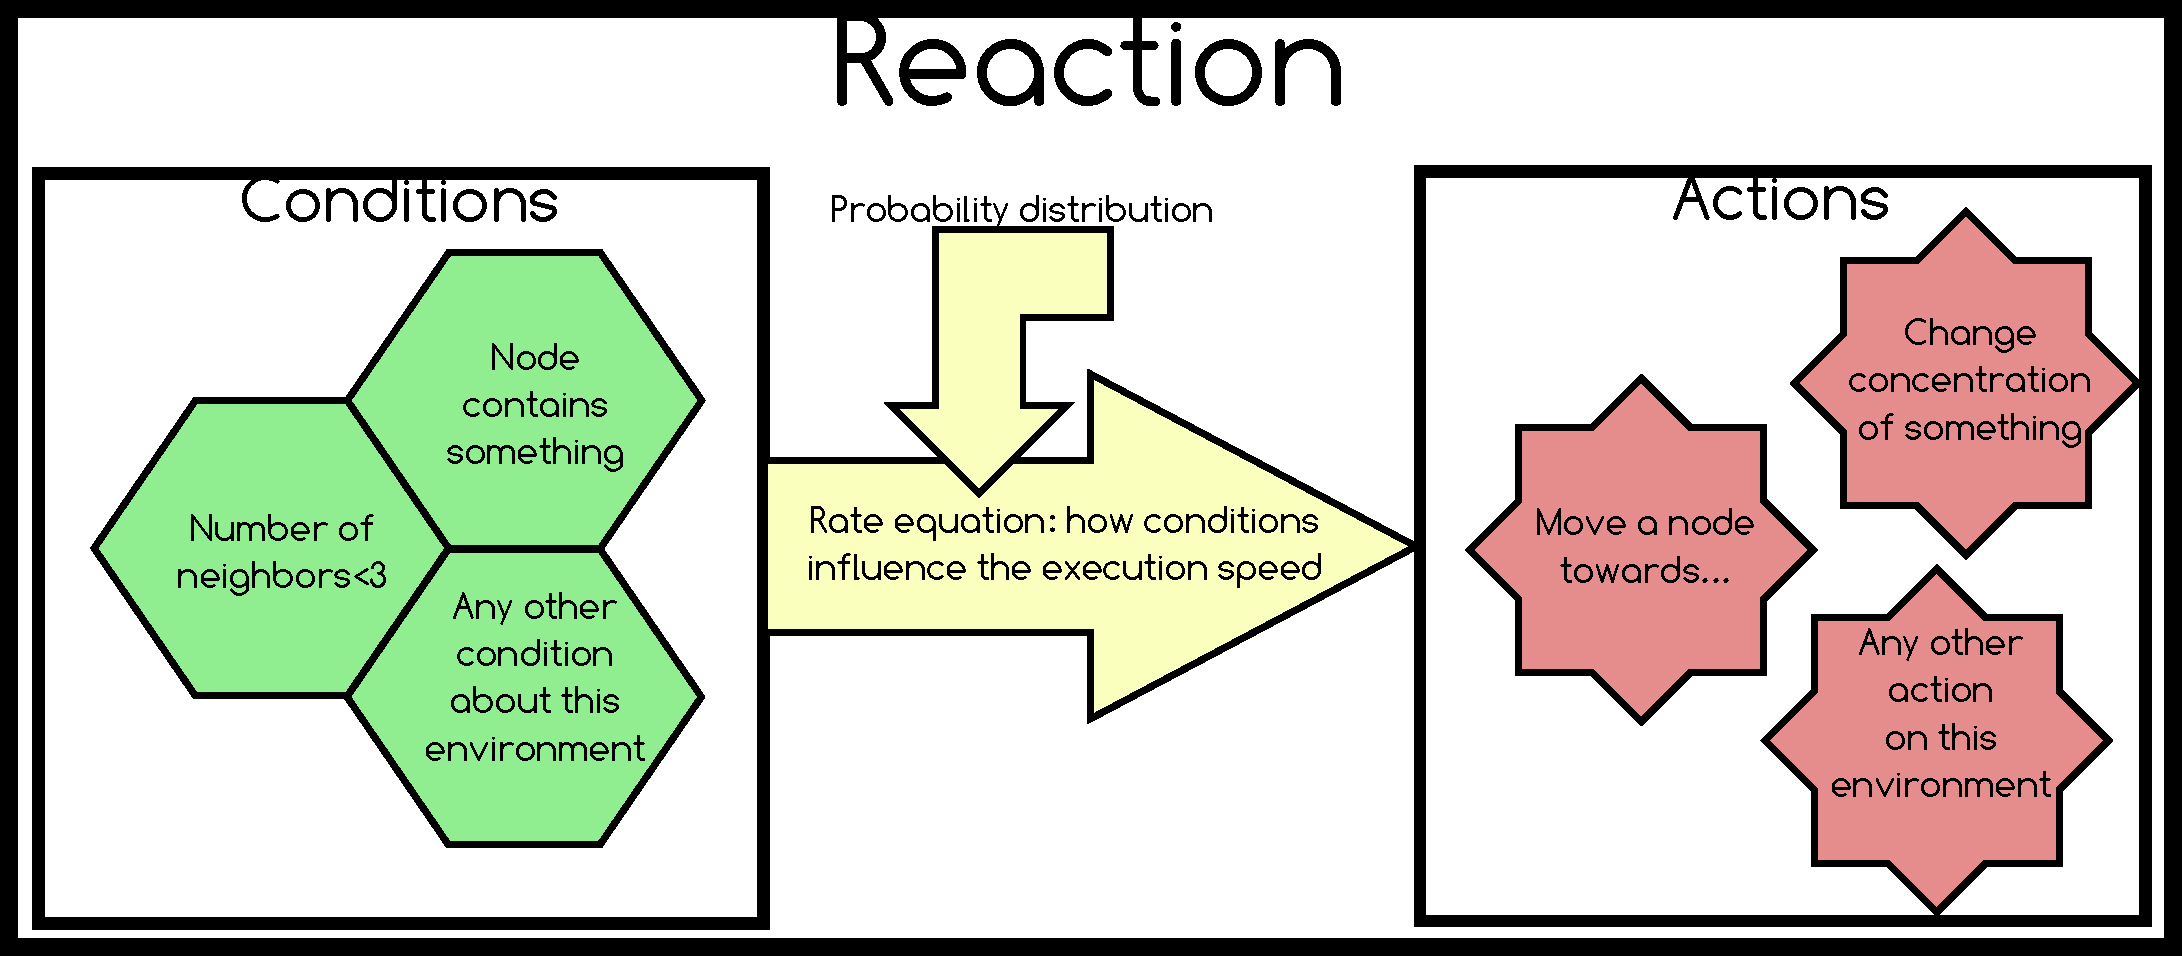
\includegraphics[width=0.99\textwidth]{img/reaction}
\end{frame}

\subsection{Architecture}
\begin{frame}{Architecture}
  \centering
  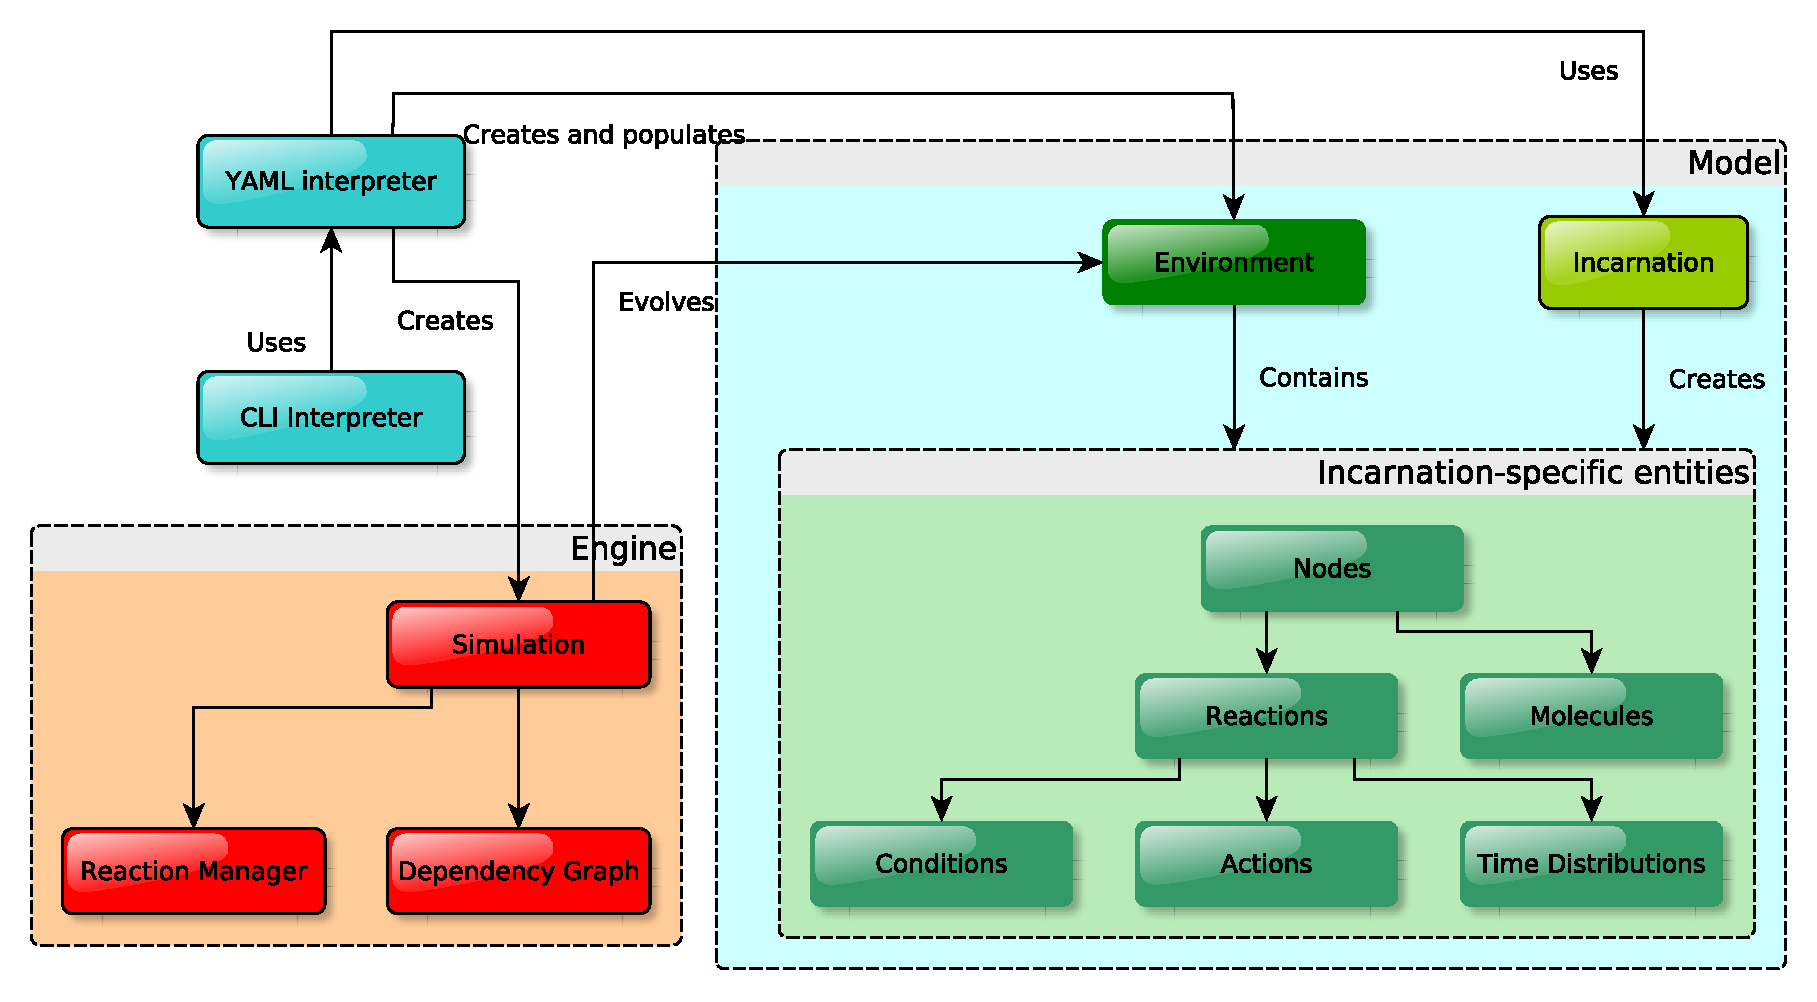
\includegraphics[width=0.99\textwidth]{img/structure}
\end{frame}

% \subsection{Performance}
% \begin{frame}{Against Repast}
%   \centering
%   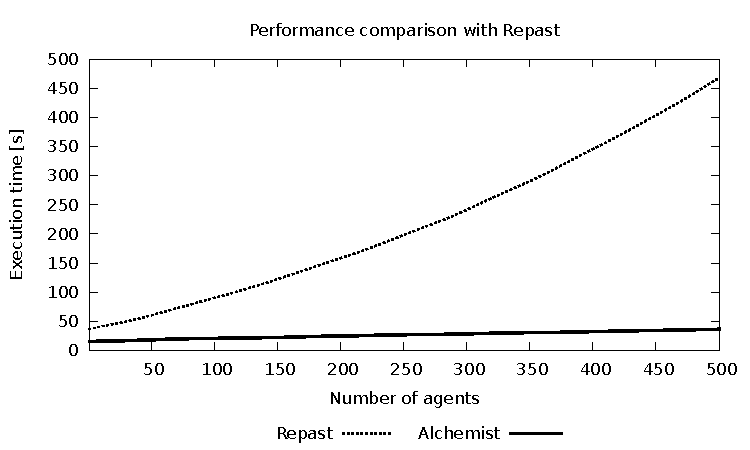
\includegraphics[width=0.99\textwidth]{img/graph01}
% \end{frame}
% 
\subsection{Sapere incarnation}
\begin{frame}{SAPERE incarnation}
 \begin{block}{Motivation}
  \begin{itemize}
   \item Alchemist was initially developed within the SAPERE Project (\url{http://www.sapere-project.eu/})
   \item At the model level, captures the required abstractions of a SAPERE system
  \end{itemize}
 \end{block}
 \begin{block}{Details on the incarnation}
  \begin{itemize}
   \item In this incarnation, the concentration is defined as ``list of tuples matching a tuple template''
   \item Basically, in this configuration Alchemist does not simulate a simple collection of intercommunicating compartments, but a network of (possibly mobile) programmable tuple spaces
   \item This one and the incarnation supporting Protelis based aggregate programming are the only two completely implemented
   \begin{itemize}
    \item there is a sketched biochemical implementation
   \end{itemize}
  \end{itemize}
 \end{block}
\end{frame}

\subsection{Simulation with the SAPERE incarnation: a mini-tutorial}

\begin{frame}{Simulating in Alchemist}
 \begin{block}{Alchemist XML}
    Alchemist 1.+ provides support for writing simulations using an XML file
  \begin{itemize}
   \item Inspired by CellML, very verbose: a file can get well over 10MB
   \item Not human friendly
   \item Each incarnation normally provides also a DSL that translates a human friendly language to the XML
   \item Considered legacy, deprecated
  \end{itemize}
 \end{block}
 \begin{block}{Alchemist YAML}
    Alchemist 2.+ adds support for writing YAML instead
  \begin{itemize}
   \item Human readable and small in size
   \item Demands creation of actual model objects to the incarnation
   \item Works for any (correctly implemented) incarnation
   \item It is still possible to write DSLs if the need arises
  \end{itemize}
 \end{block}
\end{frame}

\begin{frame}{Writing simulations with the SAPERE incarnation}
	\begin{itemize}
		\item Alchemist uses YAML as language for writing simulations
		\begin{itemize}
			\item JSON superset
			\item Compact
			\item Human-readable
			\item Supports anchoring (referencing)
		\end{itemize}
		\item The same syntax can be used for any incarnation
		\item Support for running batches
		\item No intermediate compilation
		\item No large files involved
	\end{itemize}
\end{frame}

\newcommand{\saperesimsize}[2]{
    \IfFileExists{#1.yml}{}{
        \write18{curl https://raw.githubusercontent.com/AlchemistSimulator/SAPERE-incarnation-tutorial/master/src/main/yaml/#1.yml --output #1.yml}
    }
    \inputminted[fontsize=#2,linenos=true,breaklines=true, frame=single]{yaml}{#1.yml}
}
\newcommand{\saperesim}[1]{\saperesimsize{#1}{\scriptsize}}

\begin{frame}[fragile]{Minimal specification}
	\saperesimsize{00-minimal}{\normalsize}
\end{frame}

\begin{frame}[fragile]{Node displacement and connection}
	\saperesim{01-nodes}
\end{frame}

\begin{frame}[fragile]{Multiple nodes}
	\saperesim{02-manynodes}
\end{frame}

\begin{frame}[fragile]{Grid of nodes}
	\saperesim{03-grid}
\end{frame}

\begin{frame}[fragile]{Irregular grid of nodes}
	\saperesim{04-perturb-grid}
\end{frame}

\begin{frame}[fragile]{Initial node content}
	\saperesim{05-content}
\end{frame}

\begin{frame}[fragile]{Programming nodes}
	\saperesimsize{06-send}{\tiny}
\end{frame}

\begin{frame}[fragile]{Code reuse in YAML}
	\saperesim{07-yaml-vars}
\end{frame}

\begin{frame}[fragile]{Diffusion}
	\saperesim{09-diffuse} 
\end{frame}

\begin{frame}[fragile]{Mathematical operations}
	\saperesimsize{11-math-grad}{\tiny}
\end{frame}

\begin{frame}[fragile]{Synthetic variables}
\begin{itemize}
 \item \#ID -- unique id for each LSA
 \item \#NODE -- this node id
 \item \#O -- the ``orientation'', namely the node id of the local node when an operation involving the neighborhood is performed
 \item \#D -- distance with the neighbor
 \item \#T -- current time
 \item \#RANDOM -- a random number
 \item \#NEIGHBORHOOD -- list of all neighbors ids
 \item \#SELECTEDNEIGH -- neighbor selected when performing a ``+'' operation
 \item \#ROUTE -- distance using routes, only works with maps
\end{itemize}
\end{frame}

\begin{frame}[fragile]{Personalised time distribution}
	\saperesimsize{13-timedistribution}{\tiny}
\end{frame}

\begin{frame}[fragile]{Personalised time distribution}
	Considerations:
	\begin{itemize}
		\item The syntax is a shortcut for the desired Java class' constructor
		\item You can implement your own classes implementing \texttt{TimeDistribution} and model arbitrary distributions
		\item Alchemist is a discrete-event simulator: events are forced to be ordered, even if they happen at the same time.
		\item The same syntax (a YAML map with \texttt{type} and \texttt{parameters} key) can be used to load arbitrary implementations of any simulation element
		\item The Alchemist loader automatically assigns values to arguments of type \texttt{Environment}, \texttt{Incarnation}, \texttt{RandomGenerator}, \texttt{Node}, \texttt{Reaction}, \texttt{TimeDistribution} depending on the context, letting the user specifying only the parts strictly required.
	\end{itemize}
\end{frame}

\begin{frame}[fragile]{The \texttt{variables} section}
	\saperesimsize{14-yaml-vars}{\tiny}
\end{frame}

\begin{frame}[fragile]{Variables in Alchemist}
	\begin{itemize}
	  \item Variables can be defined in a \texttt{variable} section
	  \item They are implementations of the \texttt{Variable} interface
	  \item Very useful for running batches
	  \item They can be specified as dependent variables by indicating a formula (that will then be interpreted by an internal Javascript engine)
	\end{itemize}
\end{frame}


\begin{frame}[fragile]{Movement}
	(Complete version on the provided code)
	\saperesimsize{15-move}{\tiny}
\end{frame}

\begin{frame}[fragile]{Non exhaustive Alchemist UI keyboard shortcuts}
	\begin{itemize}
	  \item[P] Pause/play
	  \item[L] enables and disables link painting
	  \item[R] Enables and disables realtime mode: tries to sync the simulation with the real time, always ensuring at least 25fps.
	  \item[$\rightarrow{}$] Makes the simulation faster (less update calls to the UI)
	  \item[$\leftarrow{}$] Makes the simulation slower (more update calls to the UI)
	  \item[M] Turns on and off the graphical marker for the node closest to the mouse pointer
	  \item[S] Enters select mode (nodes can be selected)
	  \item[O] When in select mode, enables manual move mode for selected nodes
	\end{itemize}
\end{frame}


\begin{frame}[allowframebreaks]
  \frametitle{Bibliography}
  \bibliographystyle{apalike}
  \bibliography{bib}
\end{frame}


\end{document}
